\begin{figure*}[tbhp]
    \centering
    \begin{subfigure}[t]{2.85in}
       \centering
       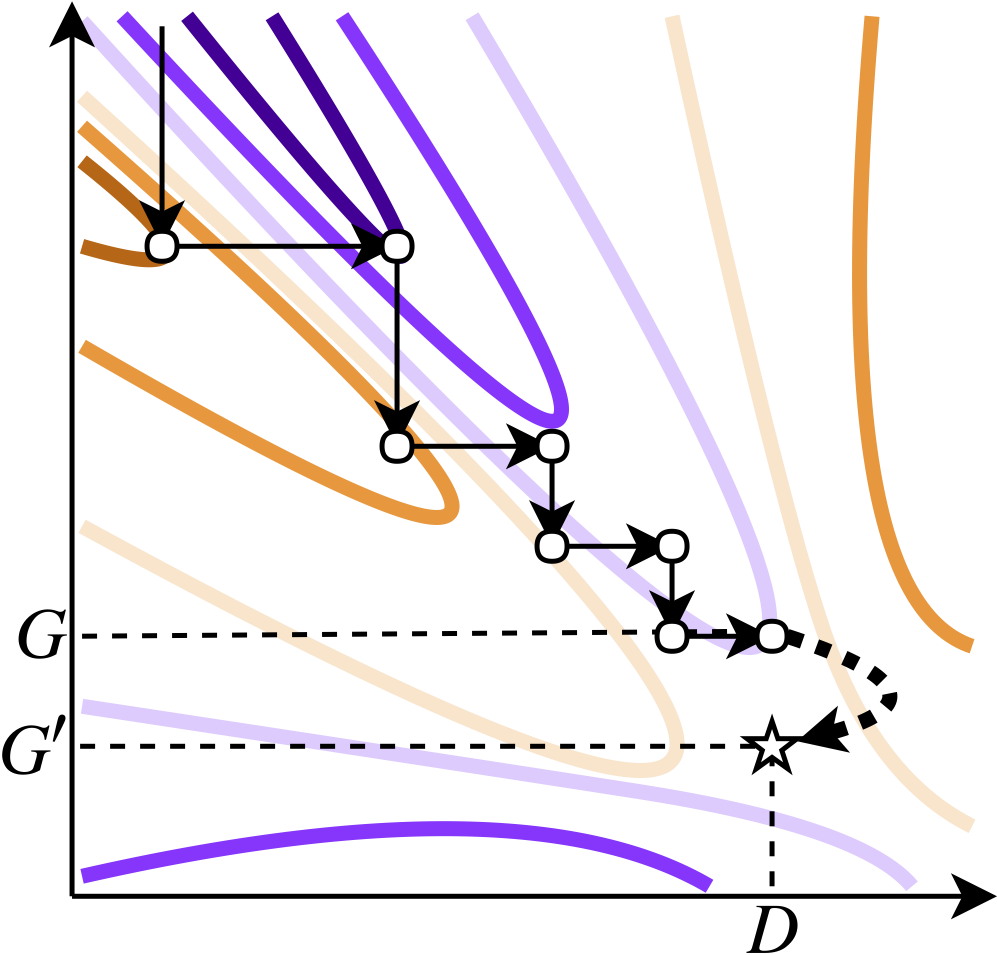
\includegraphics[scale=1.075]{figures/coord_descent.png}
       \caption{GAN value function}
    \end{subfigure}
    \hfill
    \begin{subfigure}[t]{3.8in}
       \centering
       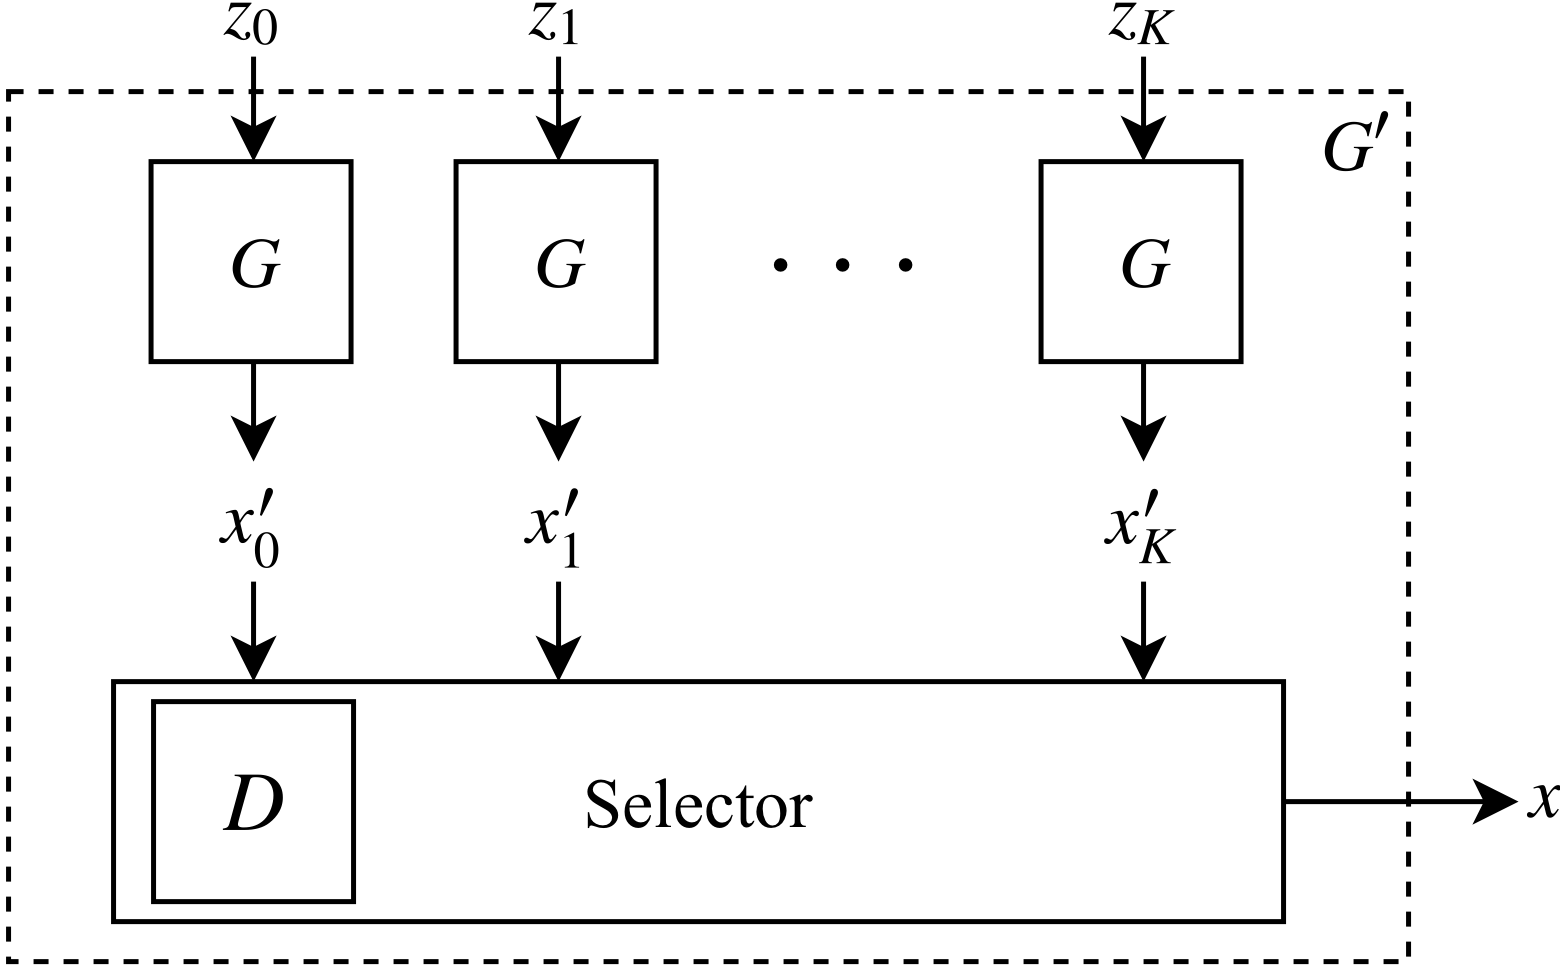
\includegraphics[scale=1.075]{figures/block_diag.png}
       \caption{$G'$ wraps $G$}
    \end{subfigure}
    \caption{{\small
    \textbf{(a)} We diagram how training of $D$ and $G$ in GANs performs coordinate descent on the joint minimax value function, shown in the solid black arrow.
    If GAN training produces a perfect $D$ for an imperfect $G$, the MH-GAN wraps $G$ to produce a perfect generator $G'$, as shown in the final dashed arrow.
    The generator $G$ moves vertically towards the orange region while the discriminator $D$ moves horizontally towards the purple.
    \textbf{(b)} We illustrate how the MH-GAN is essentially a selector from multiple draws of $G$.
    In the MH-GAN, the selector is built using a Metropolis-Hastings (MH) acceptance rule from the discriminator scores $D$.
    }}
    \label{fig:intro}
\end{figure*}
